\documentclass[11pt]{article}
\usepackage{homework}

\classname{364}
\homeworknum{1}

\DeclareSIUnit{\year}{yr}


\begin{document}

% Environments

\newcommand{\state}[2]{\begin{statement}{#1} #2 \end{statement}}
\newcommand{\prob}[2]{\begin{problem}{#1} #2 \end{problem}}
\newcommand{\subprob}[1]{\begin{subproblem} #1 \end{subproblem}}
\newcommand{\sol}[1]{\begin{solution} #1 \end{solution}}
\newcommand{\fig}[2]{\begin{figure} \centering #2  \label{#1} \end{figure}}

\newcommand{\makebib}{
	\vfill
	\color{black}
	\nocite{*}
	\bibliography{references}{}
	\bibliographystyle{lucas_unsrt}
}
	

% Implication

\newcommand{\qwhere}{\quad \text{where} \quad}
\newcommand{\qimplies}{\quad \implies \quad}
\newcommand{\impliesq}{\implies \quad}



% Brackets

\newcommand{\paren}[1]{\left( #1 \right)}
\newcommand{\brac}[1]{\left[ #1 \right]}
\newcommand{\curly}[1]{\left\{ #1 \right\}}


% Greek

\newcommand{\alp}{\alpha}
\newcommand{\bet}{\beta}
\newcommand{\gam}{\gamma}
\newcommand{\del}{\delta}
\newcommand{\eps}{\epsilon}
\newcommand{\zet}{\zeta}
\newcommand{\tht}{\theta}
\newcommand{\kap}{\kappa}
\newcommand{\lam}{\lambda}
\newcommand{\sig}{\sigma}
\newcommand{\ups}{\upsilon}
\newcommand{\omg}{\omega}

\newcommand{\Gam}{\Gamma}
\newcommand{\Del}{\Delta}
\newcommand{\Tht}{\Theta}
\newcommand{\Lam}{\Lambda}
\newcommand{\Sig}{\Sigma}
\newcommand{\Omg}{\Omega}


% Text

\newcommand{\where}{\text{where }}

% Problem 1

\newcommand{\Hint}{H_\text{int}}
\newcommand{\ddcx}{\dd[3]{x}}
\newcommand{\psib}{\bar{\psi}}

\newcommand{\mh}{m_h}
\newcommand{\mmu}{m_\mu}
\newcommand{\me}{m_e}
\newcommand{\ma}{m_a}

\newcommand{\aexpt}{a_\text{expt.}}
\newcommand{\aQED}{a_\text{QED}}
\renewcommand{\GeV}{\giga\electronvolt}

\newcommand{\gamt}{\gam^5}



\state{}{
	Let $T$ be a rank one tensor which takes as argument vectors in a finite-dimensional vector space equipped with an inner product (either Euclidean with all spacelike directions or Lorenztian with one timelike direction).  Prove that there exists a vector $V$ such that for all vectors W,
	\eq{
		\TW = V \cdot W.
	}
}





\state{Relativistic gravitational force law (MCP 2.4)}{
	In Newtonian theory, the gravitational potential $\Phi$ exerts a force $\bF = \dv*{\bp}{t} = -m \grad \Phi$ on a particle with mass $m$ and momentum $\bp$.  Before Einstein formulated general relativity, some physicists constructed relativistic theories of gravity in which a Newtonian-like scalar gravitational field $\Phi$ exerted a 4-force $\vF = \dv*{\vp}{\tau}$ on any particle with rest mass $m$, 4-velocity $\vuu$, and 4-momentum $\vp = m \vuu$.  What must that force law have been for it to (i) obey the Principle of Relativity, (ii) reduce to Newton's law in the nonrelativistic limit, and (iii) preserve the particle's rest mass as time passes?
}





\clearpage
\newcommand{\tht}{\theta}
\newcommand{\thtxx}{\tht_{xx}}
\newcommand{\thtyy}{\tht_{yy}}
\newcommand{\thttt}{\tht_{tt}}
\newcommand{\thtt}{\tht_t}
\newcommand{\thtx}{\tht_x}
\newcommand{\thty}{\tht_y}
\newcommand{\sint}{\sin{\tht}}
\newcommand{\dxdydt}{\dxdy \dd{t}}

\begin{statement}{}
	The nondimensionalized, multidimensional Sine-Gordon equation,
	\beq
		\thtxx + \thtyy - \thttt = \sint
	\eeq
	for $\tht(x, y, t)$, is the Euler-Lagrange equation for the action integral
	\beq
		S[\tht] = \intR \left\{ \frac{1}{2} \left[ \thtt^2 - (\nabla\tht)^2 \right] - \sint \right\} \dxdydt
	\eeq
	with $\nabla\tht = (\pdv*{\tht}{x}, \pdv*{\tht}{y})$.  The functional $S[\tht]$ is invariant under translation of $x$, $y$, and $t$.  Find the associated energy-momentum tensor and energy-momentum vector.
\end{statement}

\begin{solution}
	Expanding out $(\nabla\tht)^2$, the Lagrangian density is
	\beqn \label{lagr3}
		\Ld = \frac{1}{2} (\thtt^2 - \thtx^2 - \thty^2) - \sint.
	\eeqn
	The energy-momentum tensor is defined by
	\beq
		T_{ij} = \pdv{\Ld}{\tht_{x_i}} \pdv{\tht}{x_j} - \Ld \, \delta_{ij},
	\eeq
	where $x_i \in \{ x_0, x_1, x_2 \} = \{ t, x, y \}$.  The diagonal elements of $T$ are then
	\begin{align*}
		T_{00} &= \pdv{\Ld}{\thtt} \pdv{\tht}{t} - \Ld = \thtt^2 - \frac{1}{2} (\thtt^2 - \thtx^2 - \thty^2) + \sint = \frac{1}{2} (\thtt^2 + \thtx^2 + \thty^2) + \sint, \\
		T_{11} &= \pdv{\Ld}{\thtx} \pdv{\tht}{x} - \Ld = -\thtx^2 - \frac{1}{2} (\thtt^2 - \thtx^2 - \thty^2) + \sint = -\frac{1}{2} (\thtt^2 + \thtx^2 - \thty^2) + \sint, \\
		T_{22} &= \pdv{\Ld}{\thty} \pdv{\tht}{y} - \Ld = -\thty^2 - \frac{1}{2} (\thtt^2 - \thtx^2 - \thty^2) + \sint = -\frac{1}{2} (\thtt^2 - \thtx^2 + \thty^2) + \sint,
	\end{align*}
	and the nondiagonal elements are
	\begin{align*}
		T_{01} &= \pdv{\Ld}{\thtt} \pdv{\tht}{x} = \thtt \thtx, &
		T_{02} &= \pdv{\Ld}{\thtt} \pdv{\tht}{y} = \thtt \thty, &
		T_{12} &= \pdv{\Ld}{\thtx} \pdv{\tht}{y} = -\thtx \thty, \\
		T_{10} &= \pdv{\Ld}{\thtx} \pdv{\tht}{t} = -\thtt \thtx, &
		T_{20} &= \pdv{\Ld}{\thty} \pdv{\tht}{t} = -\thtt \thty, &
		T_{21} &= \pdv{\Ld}{\thty} \pdv{\tht}{x} = -\thtx \thty.
	\end{align*}
	In matrix form, we have
	\beq
		T = \mqty[(\thtt^2 + \thtx^2 + \thty^2) / 2 + \sint & \thtt \thtx & \thtt \thty \\
				-\thtt \thtx & -(\thtt^2 + \thtx^2 - \thty^2) / 2 + \sint & -\thtx \thty \\
				-\thtt \thty & -\thtx \thty & -(\thtt^2 - \thtx^2 + \thty^2) / 2 + \sint ].
	\eeq
	The energy-momentum vector is defined by
	\beq
		P_j = \int T_{0j} \dd{x_1} \dd{x_2}.
	\eeq
	Its components are then
	\begin{align*}
		P_0 &= \int \left[ \frac{1}{2} (\thtt^2 + \thtx^2 + \thty^2) + \sint \right] \dxdy, &
		P_1 &= \int \thtt \thtx \dxdy, &
		P_2 &= \int \thtt \thty \dxdy.
	\end{align*}
\vfix
\end{solution}






\clearpage
\state{Spacetime diagrams (MCP 2.14)}{ \label{4}
	Use spacetime diagrams to prove the following.
}

\begin{figure}[p] \centering
	\begin{tabular}{c c}
		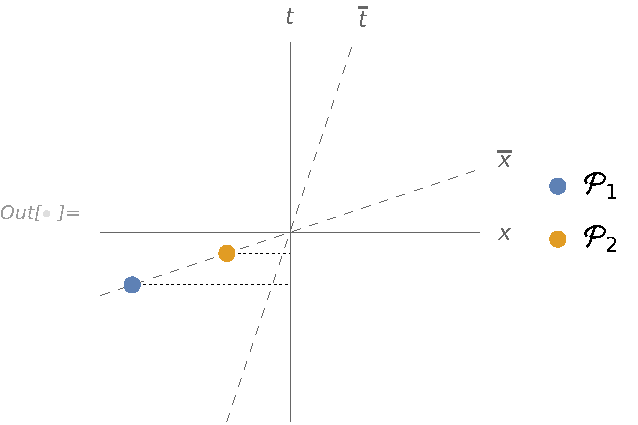
\includegraphics[trim=1.5cm 0 0 0,clip]{4a} &
		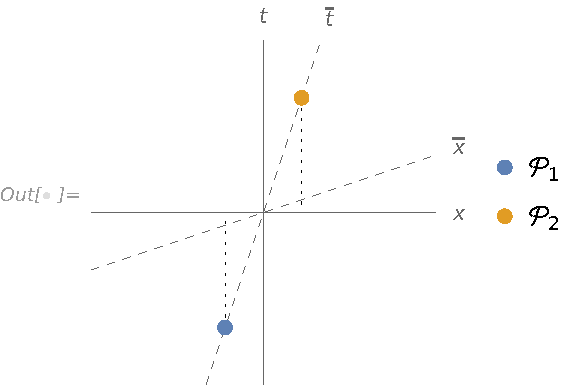
\includegraphics[trim=1.5cm 0 0 0,clip]{4b} \\
		(a) & (b) \\[2ex]
		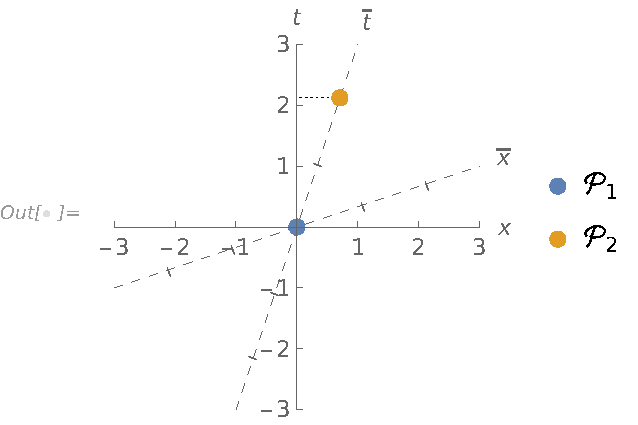
\includegraphics[trim=1.5cm 0 0 0,clip]{4c} &
		\\
		(c) & (d) \\[2ex]
		\\
		(e) & (f) \\
	\end{tabular}
	\caption{Spacetime diagrams for problem~\ref{4}.}
	\label{f4}
\end{figure}

\prob{
	Two events that are simultaneous in one inertial frame are not necessarily simultaneous in another.  More specifically, if frame $\cFb$ moves with velocity $\vv = \bet \vex$ as seen in frame $\cF$, where $\bet > 0$, then of two events that are simultaneous in $\cFb$ the one farther ``back'' (with the more negative value of $\xb$) will occur in $\cF$ before the one farther ``forward.''
}

\sol{
	Figure~\ref{4}~(a) shows a spacetime diagram for frames $\cF$ and $\cFb$.  Two events, $\cPq$ and $\cPw$, are located on the $\xb$ axis.  In $\cFb$, they occur simultaneously at $\tb = 0$.  The dotted lines extending from the events to the $t$ axis show when the events occur in $\cF$.  Event $\cPq$ is farther back and occurs earlier in $\cF$ than event $\cPw$.  Thus two events that are simultaneous in $\cFb$ are not simultaneous in $\cF$. \qed
}



\prob{
	Two events that occur at the same spatial location in one inertial frame do not necessarily occur at the same spatial location in another.
}

\sol{
	Figure~\ref{4}~(b) shows a spacetime diagram in which events $\cPq$ and $\cPw$ both occur at position $\xb = 0$ in $\cFb$.  The dotted lines extending from the events to the $x$ axis show that, in $\cF$, event $\cPq$ occurs at $x < 0$ and event $\cPw$ at $x > 0$.  Hence, the events do not occur at the same position in $\cF$. \qed
}



\prob{
	If $\cPq$ and $\cPw$ are two events with a timelike separation, then there exists an inertial reference frame in which they occur at the same spatial location, and in that frame the time lapse between them is equal to the square root of the negative of their invariant interval, $\Del t = \Del \tau \equiv \sqrt{-(\Del s)^2}$.
}

\sol{
	Figure~\ref{4}~(c) shows a spacetime diagram in which the $t$ and $x$ axes are given arbitrary units.  Events $\cPq$ and $\cPw$ occur at the same location in $\cF$, $x = 2$.  The dotted lines in Fig.~\ref{4}~(c) show the $(\tb, \xb)$ coordinates of $\cPq$ and $\cPw$.  Their $\Del \tb$ is greater than their $\Del \xb$, so their separation is clearly timelike in $\cFb$ as well.
	
	The interval, which is invariant of reference frame, can be calculated in one spatial and one temporal dimension by adapting (2.2a) in MCP:
	\eqn{interval}{
		(\Del s)^2 = -(\Del t)^2 + (\Del x)^2.
	}
	In $\cF$, $\Del x = 0$ and $\Del t = 2$.  Then
	\eq{
		(\Del s)^2 = -2^2 + 0^2
		= -4
		< 0,
	}
	so the interval is indeed timelike~\cite[p.~45]{MCP}.  Since the events are at the same spatial location in $\cF$, we calculate the time lapse between them in $\cF$ as
	\eq{
		\sqrt{-(\Del s)^2} = \sqrt{4} = 2,
	}
	which is exactly as shown in the figure. \qed
}



\prob{
	If $\cPq$ and $\cPw$ are two events with a spacelike separation, then there exists an inertial reference frame in which they are simultaneous, and in that frame the spatial distance between them is equal to the square root of their invariant interval, $\sqrt{\gij \Del \xii \Del \xj} = \Del s \equiv \sqrt{(\Del s)^2}$.
}



\prob{
	If the inertial frame $\cFb$ moves with speed $\bet$ relative to the frame $\cF$, then a clock at rest in $\cFb$ ticks more slowly as viewed from $\cF$ than as viewed from $\cFb$---more slowly by a factor $\gam^{-1} = \sqrt{1 - \bet^2}$.  This is called \emph{relativistic time dilation}.  As one consequence, the lifetimes of unstable particles moving with a speed $\bet$ are increased by the Lorentz factor $\gam$.
}


\prob{
	If the inertial frame $\cFb$ moves with velocity $\vv = \bet \vex$ relative to the frame $\cF$, then an object at rest in $\cFb$ as studied in $\cF$ appears shortened by a factor $\gam^{-1} = \sqrt{1 - \bet^2}$ along the $x$ direction, but its length along the $y$ and $z$ directions is unchanged.  This is called \emph{Lorentz contraction}.  As one consequence, heavy ions moving at high speeds in a particle accelerator appear to act like pancakes, squashed along their directions of motion.
}





\clearpage
\state{Twins paradox (MCP 2.16)}{\hfix}

\prob{
	The 4-acceleration of a particle or other object is defined by $\vaa \equiv \dv*{\vuu}{\tau}$, where $\vuu$ is its 4-velocity and $\tau$ is proper time along its world line.  Show that, if an observer carries an accelerometer, the magnitude $\abs{\ba}$ of the 3-dimensional acceleration $\ba$ measured by the accelerometer will always be equal to the magnitude of the observer's 4-acceleration, $\abs{\ba} = \abs{\vaa} \equiv \sqrt{\vaa \cdot \vaa}$.
}


\prob{
	In the twins paradox of Fig.~2.8a, suppose that Florence begins at rest beside Methuselah, then accelerates in Methuselah's $x$-direction with an acceleration $a$ equal to one Earth gravity, $g$, for a time $\TFlo / 4$ as measured by her, then accelerates in the $-x$-direction at $g$ for a time $\TFlo / 2$, thereby reversing her motion; then she accelerates in the $+x$-direction at $g$ for a time $\TFlo / 4$, thereby returning to rest beside Methuselah.  (This is the type of motion shown in the figure.)  Show that the total time lapse as measured by Methuselah is
	\eq{
		\TMet = \frac{4}{g} \sinh(\frac{g \TFlo}{4}).
	}
}


\prob{
	Show that in the geometrized units used here, Florence's acceleration (equal to acceleration of gravity at the surface of Earth) is $g = \SI{1.033}{\per\year}$.  Plot $\TMet$ as a function of $\TFlo$, and from your plot estimate $\TFlo$ if $\TMet$ is the age of the Universe, 14 billion years.
}


\makebib

\end{document}
